\documentclass[tikz,border=5mm]{standalone}
\usepackage{tikz}
\usetikzlibrary{calc,angles}

\begin{document}
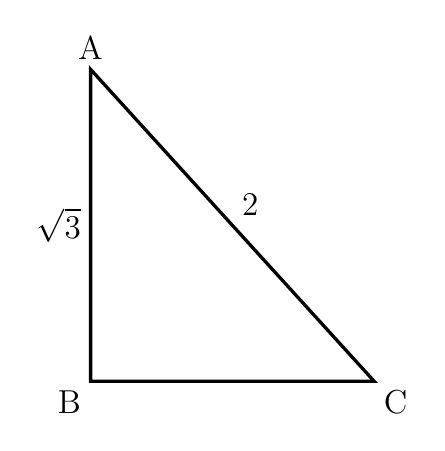
\begin{tikzpicture}[scale=1.8]

% Define vertices
\coordinate (A) at (0,2.2);
\coordinate (B) at (0,0);
\coordinate (C) at (2,0);

% Draw triangle ABC
\draw[very thick] (A) -- (B) -- (C) -- cycle;

% Vertex labels
\node[above] at (A) {\large A};
\node[below left] at (B) {\large B};
\node[below right] at (C) {\large C};

% Side labels
\node[left] at ($(A)!0.5!(B)$) {\large $\sqrt{3}$};
\node[above right] at ($(A)!0.5!(C)$) {\large $2$};

\end{tikzpicture}
\end{document}